\documentclass[a4paper, 12pt]{article}
\usepackage[utf8]{inputenc}
\usepackage[english,russian]{babel}
\usepackage[warn]{mathtext}
\usepackage{graphicx}
\usepackage{float}
\restylefloat{table}
\usepackage{amsmath}
\usepackage{floatflt}
\usepackage[T2A]{fontenc}
\usepackage[left=20mm, top=20mm, right=20mm, bottom=20mm, footskip=10mm]{geometry}

\tolerance 1414
\hbadness 1414
\emergencystretch 1.5em
\hfuzz 0.3pt        % размер максимального переполнения без warning'a
\widowpenalty=10000 % запрещает одиночную строку абзаца в начале страницы
\vfuzz \hfuzz
\raggedbottom       % если на странице мало содержимого, добавить пустое место в конце, а не в середине страницы



\begin{document}

\begin{titlepage}
	\centering
	\vspace{5cm}
	{\scshape\LARGE московский физико-технический институт (национальный исследовательский университет) \par}
	\vspace{6cm}
	{\scshape\Large Лабораторная работа 3.7.1 \par}
	{\huge\bfseries Скин-эффект в полом цилиндре \par}
	\vspace{1cm}
	\vfill
\begin{flushright}
	{\large Б03-102}\par
	\vspace{0.3cm}
	{\LARGE Куланов Александр}
\end{flushright}
	

	\vfill


	Долгопрудный, 2022 г.
\end{titlepage}

\begin{itemize}
	\item \textbf{Цель работы:} исследование проникновения переменного магнитного поля в медный полый цилиндр.
    \item \textbf{В работе используются:} генератор звуковой частоты, соленоид, намотанный на полый цилиндрический каркас из диэлектрика, медный экран в виде трубки, измерительная катушка, амперметр, вольтметр, осциллограф.
\end{itemize}

\section{Теоретические сведения}
В работе изучается Скин-эффект в длинном тонкостенном медном цилиндре, помещенном внутрь соленоида.

Теоретически такая задача сложнее, чем рассмотренный в п. 3.1 скин-эффект в полубесконечном пространстве: здесь требуется совместное решение уравнений скин-эффекта (уравнение диффузии поля)
(7.22/23) в стенке цилиндра и квазистационарных уравнений поля в его полости.

Пусть цилиндр достаточно длинныый, так что в нём можно пренебречь краевыми эффектами. В этом приближении магнитное поле H всюду направлено по оси системы, а вихревое электрическое поле E
будет всюду перпендикулярно радиусу, то есть линии поля образуют соосные окружности. Все величины будем считать колеблющимися по гармоническому закону с некоторой частотой $\omega$,
задаваемой частотой колебания тока в соленоиде. Тогда для ненулевых компонент поля можно записать 
$$ H_z = H(r)e^{i\omega t}, E_{\phi} = E(r)e^{i\omega t} $$
где H(r) и E(r) --- комплексные амплитуды колебаний соответствующих полей, зависящие только от расстояния r до оси системы. Заметим, что на границе цилиндра должны быть непрерывны
касательные к поверхности компоненты E и B, поэтому функции непрерывны во всей исследуемой области.

Пусть длинный полый цилиндр имеет радиус a и толщину стенки h << a. Последнее условие позволяет для описания полля внутри стенки ограничиться одномерным приближением. При этом 
для полного решения задачи необходимо вычислить и распределение поля внутри цилиндра.

Поскольку внутри цилиндра ток отсутствует, магнитное поле там является однородным (аналогично полю внутри пустого соленоида): $H_z(r, t) = H_1 e^{i\omega t}$, где $H_1 = const$
--- амплитуда поля на внутренней поверхности цилиндра. Для нахождения вихревого электрического поля воспользуемся законом электромагнитной индукции в интегральной форме:
$$
E_{\varphi} \cdot 2 \pi r=-\mu_0 \pi r^2 \cdot \frac{d H_z}{d t} \quad \rightarrow \quad E(r)=-\frac{1}{2} \mu_0 r \cdot i \omega H_1 .
$$
Отсюда получим связь амплитуд колебаний электрического и магнитного полей на внутренней границе цидиндра:
\begin{equation}
	E_1 = -\frac{1}{2}i\omega a \mu_0 H_1
\end{equation}

Поле внутри тонкой стенки цилиндра («экрана») описывается уравнением скин-эффекта (7.25) (уравнением диффузии поля) в плоской геометрии (рис. 2). Поместим начало отсчёта на внешнюю поверхность цилиндра и направим ось $x$ к оси системы, и аналогично (7.26) запишем дифференциальное уравнение для комплексной амплитуды магнитного поля: 
\begin{equation} 
	\frac{d^2 H}{d x^2}=i \omega \sigma \mu_0 H
\end{equation}
(для медного цилиндра можно положить $\mu \approx 1$). 

Граничные условия для (2) зададим в виде
\begin{equation}
H(0)=H_0, \quad H(h)=H_1
\end{equation}
Здесь $H_0$ - амплитуда колебаний магнитного поля на внешней границе цилиндра. Её значение определяется только током в обмотке соленоида, и совпадает с полем внутри соленоида в отсутствие цилиндра. Величина $H_1$ также поддаётся непосредственному измерению - это азплитуда колебаний однородного поля внутри цилиндра. Поля $H_0$ и $H_1$ не являются независимыми - они связаны через решение уравнений поля вне проводника, т. е. внутри «экранаэ. Эта связь выражена соотношением (1). Решение (2) ищем в виде
\begin{equation}
H(x)=A e^{\alpha x}+B e^{-\alpha x}
\end{equation}
где $A, B$ - определяемые из граничных условий константы,
\begin{equation}
\alpha=\sqrt{i \omega \sigma \mu_0}=\frac{1+i}{\delta}=\frac{\sqrt{2}}{\delta} e^{i \pi / 4}
\end{equation}
- один из корней уравнения (7.28), $\delta$ - глубина скин-слоя (7.30). Заметим, что это решение немного отличается от (7.29): ранее мы использовали только один корень уравнения (7.28), однако здесь мы имеем дело уже не с полупространством, а с конечной областью в виде плоского слоя $h$, поэтому решение должно содержать оба корня.

Первое условие (3) даёт $A+B=H_0$, тто позволяет исключить $A$ из (4):
$$
H(x)=H_0 e^{-\alpha x}+2 B \operatorname{sh} \alpha x,
$$
Выразим электрическое поле из закона Ампера (7.21), В одномерном случае
$$
E(x)=\frac{1}{\sigma} \frac{d H}{d x}=\frac{\alpha}{\sigma}\left(-H_0 e^{-\alpha x}+2 B \operatorname{ch} \alpha x\right),
$$
Делее полояим $x=h$, воспользуемся условием (1), и, исключив константу $B$ получим после преобразований связь между $H_0$ и $H_1$ :
\begin{equation}
H_1=\frac{H_0}{\operatorname{ch} \alpha h+\frac{1}{2} \alpha a \operatorname{sh}(\alpha h)}
\end{equation}
Рассмотрим предельшые случаи (6).

1. При малых частотах толщина скин-слоя превосходит толщину цилиндра $\delta \gg h$. Тогда $|\alpha h| \ll 1$, поэтому ch $\alpha h \approx 1$, sh $\alpha h \approx \alpha h$ и
\begin{equation}
	H_1 \approx \frac{H_0}{1+i \frac{a h}{\delta^2}}
\end{equation}
Заметим, что величина $a h / \delta^2$ в общем случае не мала, поскольку при $h \ll a$ возможна ситуањия $h \ll \delta \ll a$. Отношение модулей амплитуд здесь будет равио
\begin{equation}
	\frac{\left|H_1\right|}{\left|H_0\right|}=\frac{1}{\sqrt{1+\left(\frac{a h}{\delta^2}\right)^2}}=\frac{1}{\sqrt{1+\frac{1}{4}\left(a h \sigma \mu_0 \omega\right)^2}}
\end{equation}
При этом колебания $H_1$ отстают по фазе от $H_0$ на угол $\psi$, определяемый равенством $\operatorname{tg} \psi=\frac{a h}{\delta^2}$.

2. При достаточно больших частотах толщина скин-слоя станет меньше толщины стенки: $\delta \ll h$. Тогда $|\alpha h| \gg 1$ и $|\alpha a| \gg 1$, а также $\operatorname{sh}(\alpha h) \approx \operatorname{ch}(\alpha h) \approx \frac{1}{2} e^{\alpha h}$. Выражение (6) с учётом $(5)$ переходит в
\begin{equation}
\frac{H_1}{H_0}=\frac{4}{\alpha a} e^{-\alpha h}=\frac{2 \sqrt{2} \delta}{a} e^{-\frac{h}{\delta}} e^{-i\left(\frac{\pi}{4}+\frac{h}{\delta}\right)}
\end{equation}
Как видно из формулы (9), в этом пределе поле внутри цилиндра по модулю в $\frac{2 \sqrt{2} \delta}{a} e^{-h / \delta}$ раз меньше, чем снаружи, и, кроме того, запаздывает по фазе на
\begin{equation}
\psi=\frac{\pi}{4}+\frac{h}{\delta}=\frac{\pi}{4}+h \sqrt{\frac{\omega \sigma \mu_0}{2}}
\end{equation}


\section{Экспериментальная установка}
\begin{figure}[H]
    \centering
    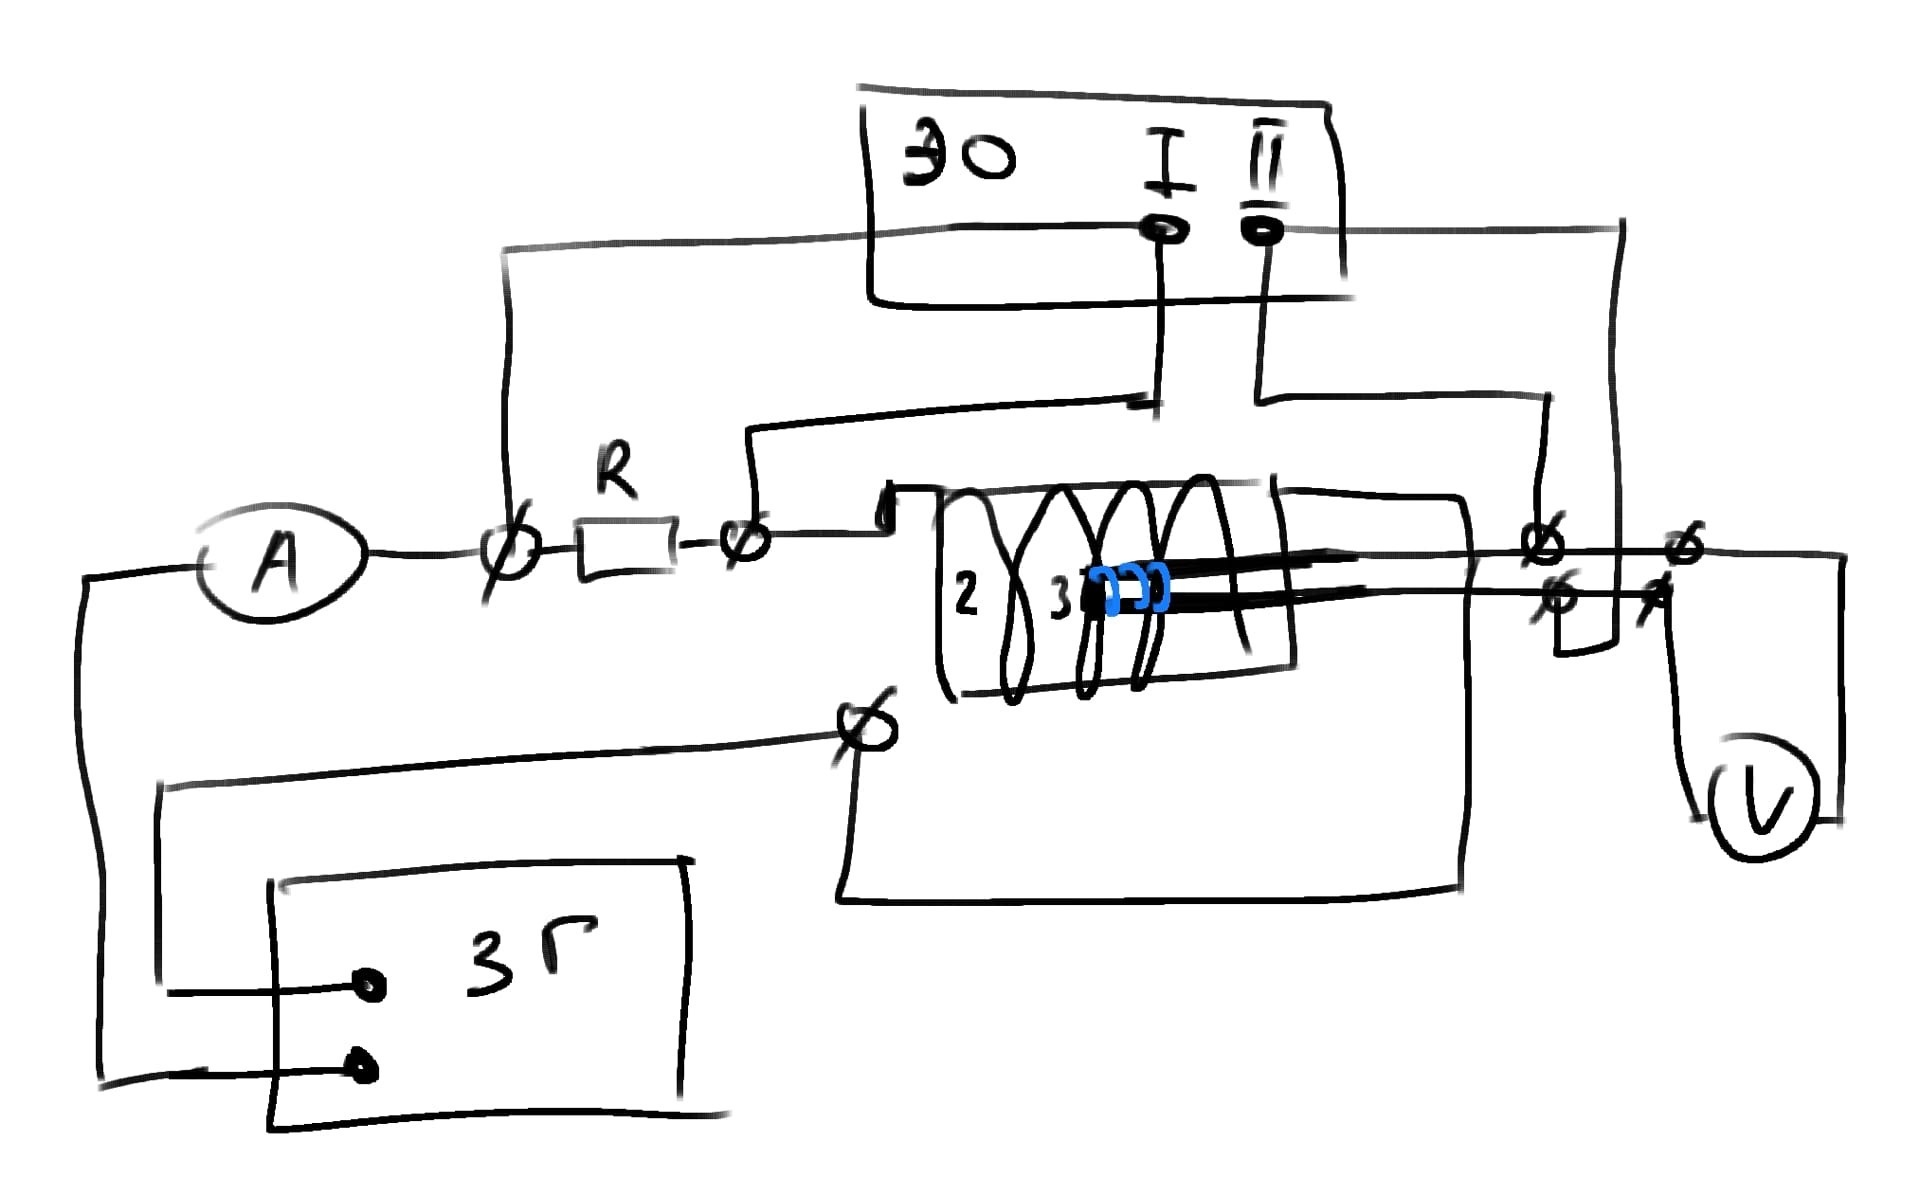
\includegraphics[width=1\textwidth]{set}
    \caption{Схема установки}
    \label{fig:set}
\end{figure}
Схема экспериментальной установки для исследования проникновения переменного магнитного поля в медный полый цилиндр изображена на рис. \ref{fig:set}. Переменное магнитное поле создаётся с помощью соленоида, намотанного на полый цилиндрический каркас 1 из поливинилхлорида, который подключается к генератору звуковой частоты. Внутри соленоида расположен медный цилиндрический экран 2. Для измерения магнитного поля внутри экрана используется измерительная катушка 3. Необходимые параметры соленоида, экрана и измерительной катушки указаны на установке. Действующее значение переменного тока в цепи соленоида измеряется амперметром $A$, а действующее значение напряжения на измерительной катушке измеряет вольтметр $V$. Для измерения сдвига фаз между током в цепи соленоида и напряжением на измерительной катушке используется двухканальный осциллограф. На вход одного канала подаётся напряжение с резистора $R$, которое пропорционально току, а на вход второго канала - напряжение с измерительной катушки.
Измерение отношения амплитуд магнитного поля внутри и вне экрана. С помощью вольтметра $V$ измеряется действующее значение ЭДС индукции, которая возникает в измерительной катушке, находящейся в переменном магнитном поле $H_1 e^{i \omega t}$. Комплексная амплитуда
ЭДС индукции в измерительной катушке равна
$$
U=-S N \frac{d B_1(t)}{d t}=-i \omega \mu_0 S N H_1 e^{i \omega t},
$$
где $S N$ - произведение площади витка на число витков измерительной катушки. Показания вольтметра, измеряющего это напряжение:
$$
U=\frac{S N \omega}{\sqrt{2}} \mu_0\left|H_1\right| .
$$
Видно, что модуль амплитуды магнитного поля внутри экрана $\left|H_1\right|$ пропорционален $U$ и обратно пропорционален частоте сигнала $\nu=\omega / 2 \pi$ :
$$
\left|H_1\right| \propto \frac{U}{\nu} .
$$
При этом поле вне экрана $\left|H_0\right|$ пропорционально току $I$ в цепи соленоида, измеряемому амперметром $A$ :
$$
\left|H_0\right| \propto I .
$$
Следовательно,
\begin{equation}
\frac{\left|H_1\right|}{\left|H_0\right|}=\text { const } \cdot \frac{U}{\nu I}
\end{equation}
Таким образом, отношение амплитуд магнитных полей снаружи и вне экрана (коэффициент ослабления) может быть измерено по отношению $U / \nu I$ при разных частотах. Неизвестная константа в соотношении (11) может быть определена по измерениям при малых частотах $\nu \rightarrow 0$, когда согласно (8) $\left|H_1\right| /\left|H_0\right| \rightarrow 1$.


\section{Обработка результатов}


\end{document}